The user interface is as follow:
\begin{itemize}
    \item{\textit{The Main Page:}} 
    \begin{figure}[!htbp]
    \begin{center}
    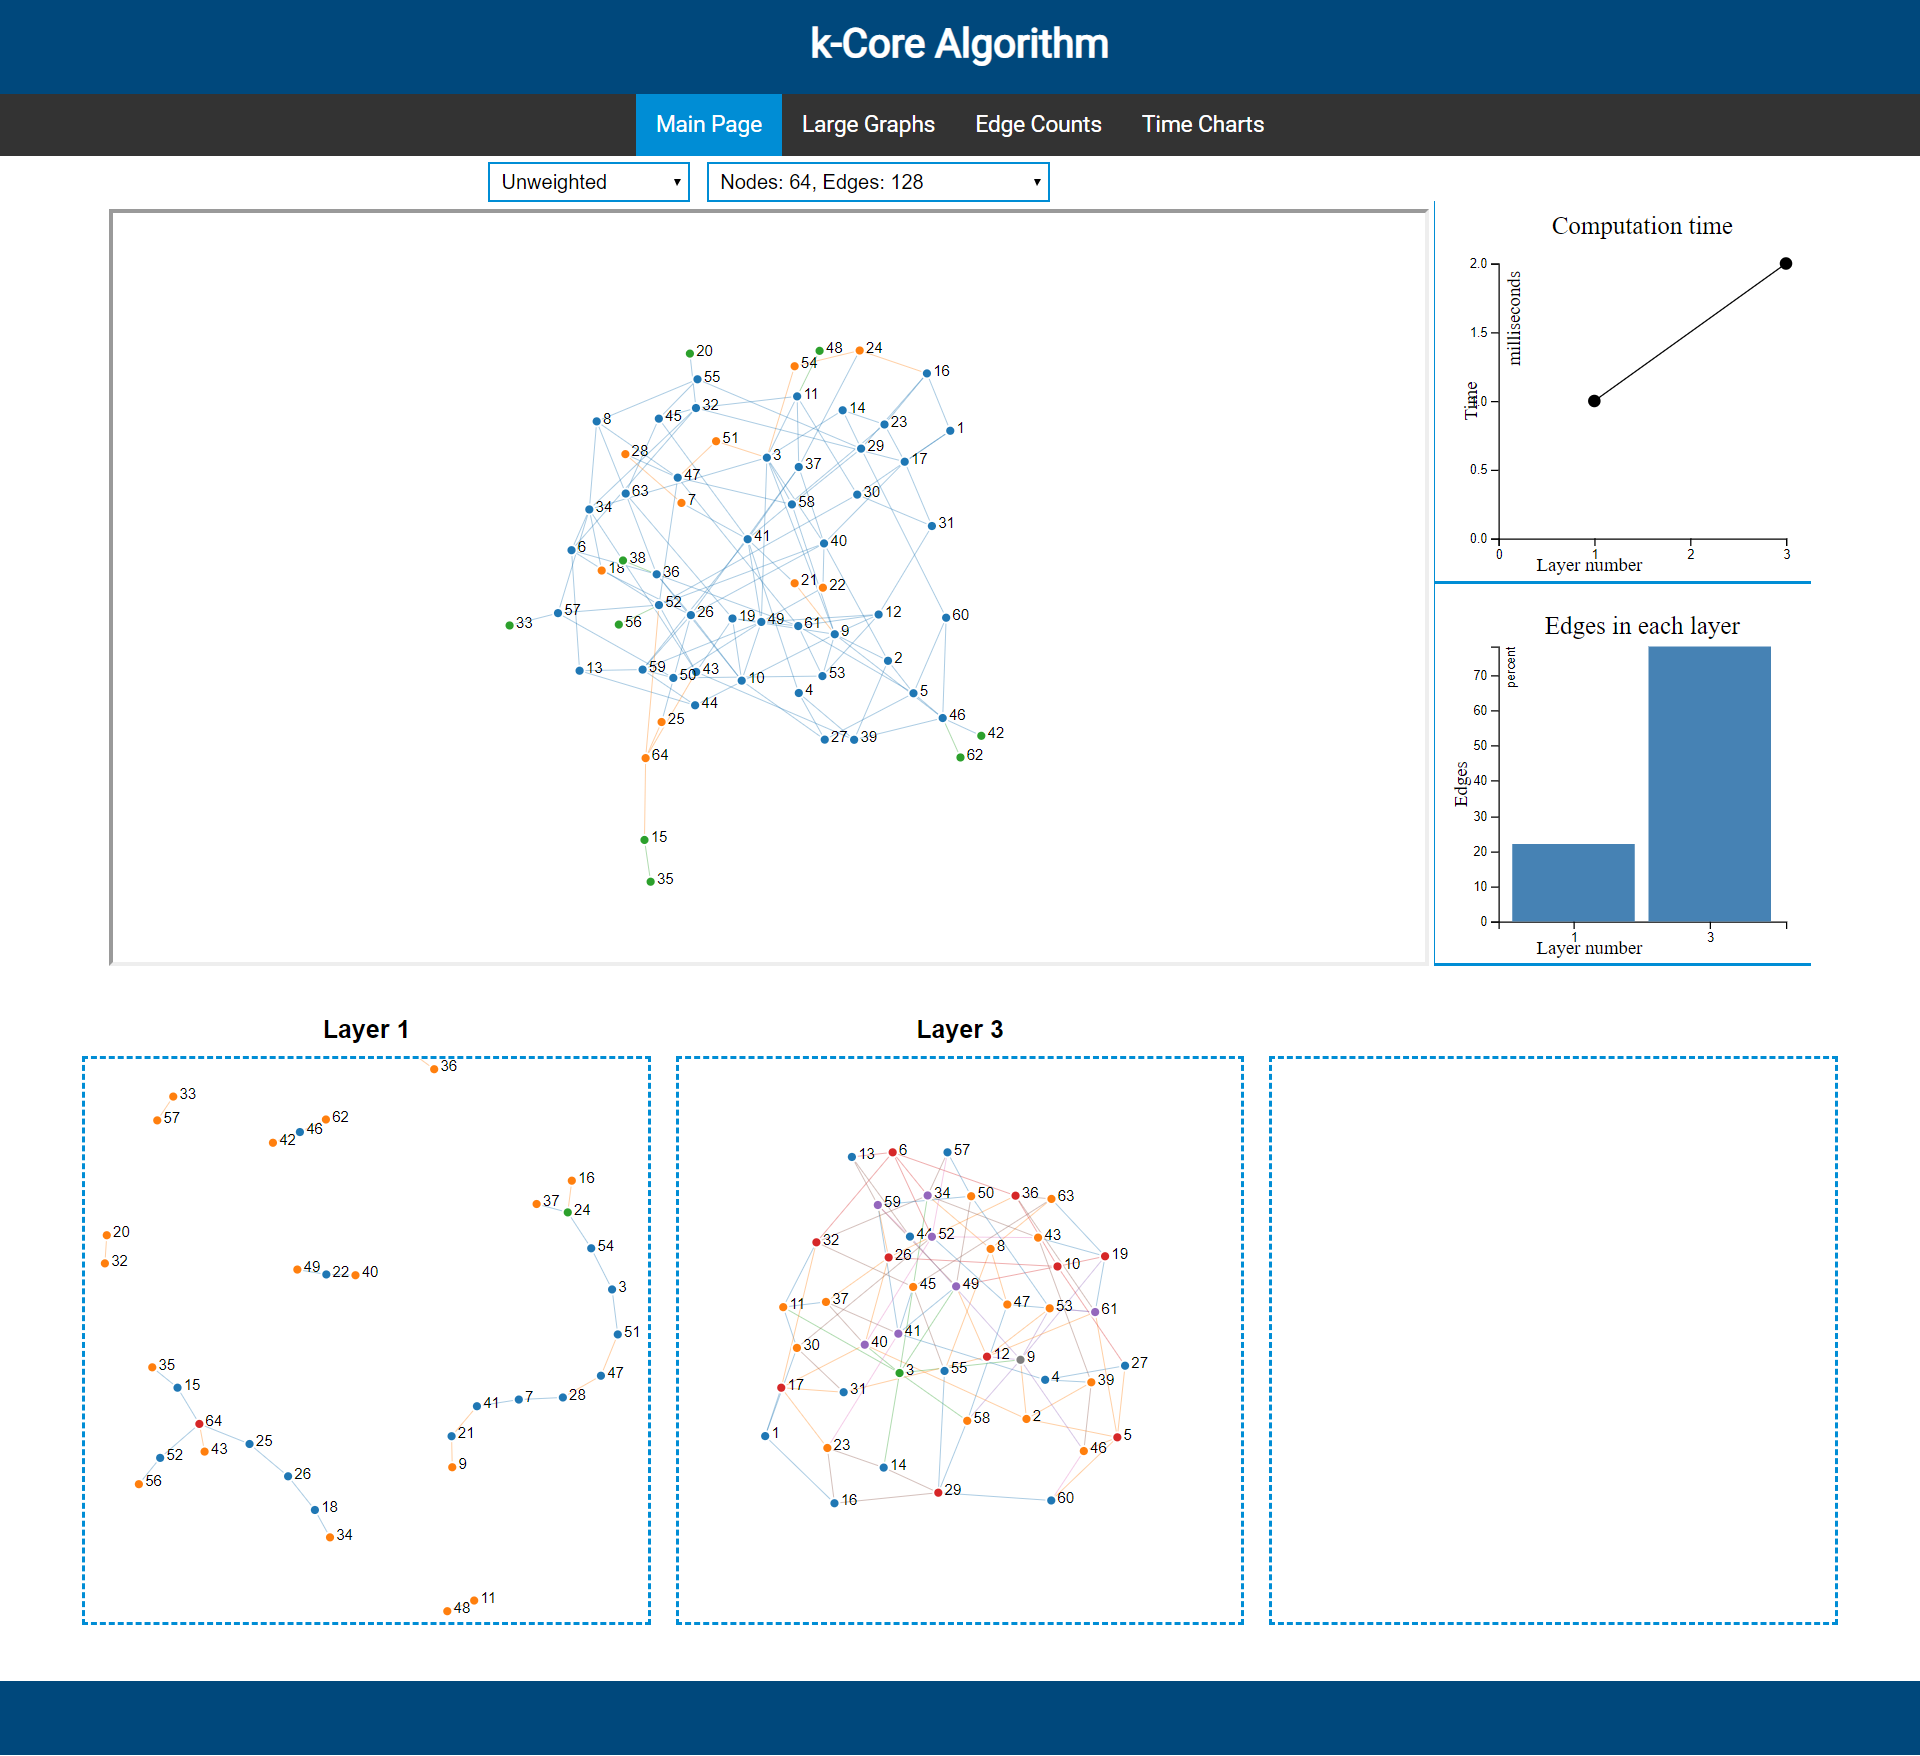
\includegraphics[width=8cm]{Final_Interface.png}
    \end{center}
    \caption{ The Main page }
    \end{figure}
    \begin{itemize}
        \item The user has the option of selecting whether they want to see the weighted graphs or the unweighted graphs. Once selected, the desired node size and edge counts can be selected from a second selector.
        \item Once a graph is selected, the corresponding bar chart depicting the concentration of edges in each layer and the computation time for each layer are displayed in a sidebar.
        \item The layers of the graph can be viewed by pressing the \textit{Layers} button at the bottom. 3 layers are generated at a time and the \textit{More Layers} button can be be pressed to generate further layers. The button will be available as long as there are further layers to be generated.
        \item When the \textit{mouseOver} action is performed on a vertex, all the neighbouring vertices of that vertex are highlighted and the remaining vertices are blurred out.
        \item When hovering over a vertex in the main graph, the core number of that vertex is shown.
        \item The graph vertices can be dragged within the graph container to better view a link or a vertex at the convenience of the user.
        \item A zoom function is also available on scroll-in/scroll-out for the user to focus on a vertex, a particular part of the graph or the graph as a whole.
    \end{itemize}
    
    \begin{figure}[!htbp]
    \begin{center}
    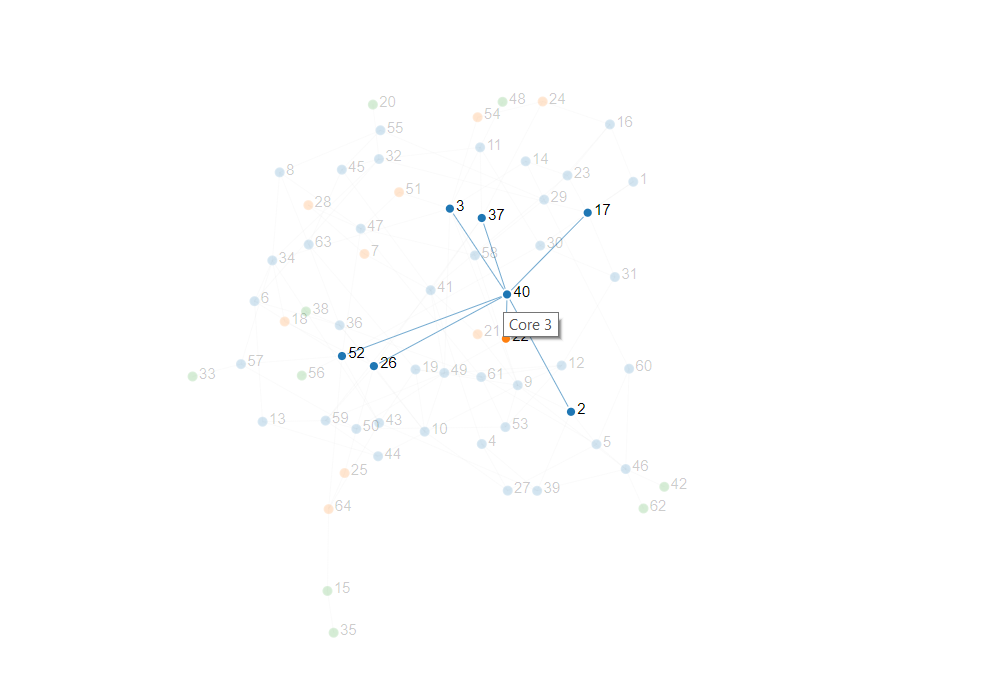
\includegraphics[width=8cm]{MouseHover.png}
    \end{center}
    \caption{ The MouseOver Effect }
    \end{figure}
    
    \begin{figure}[!htbp]
    \begin{center}
    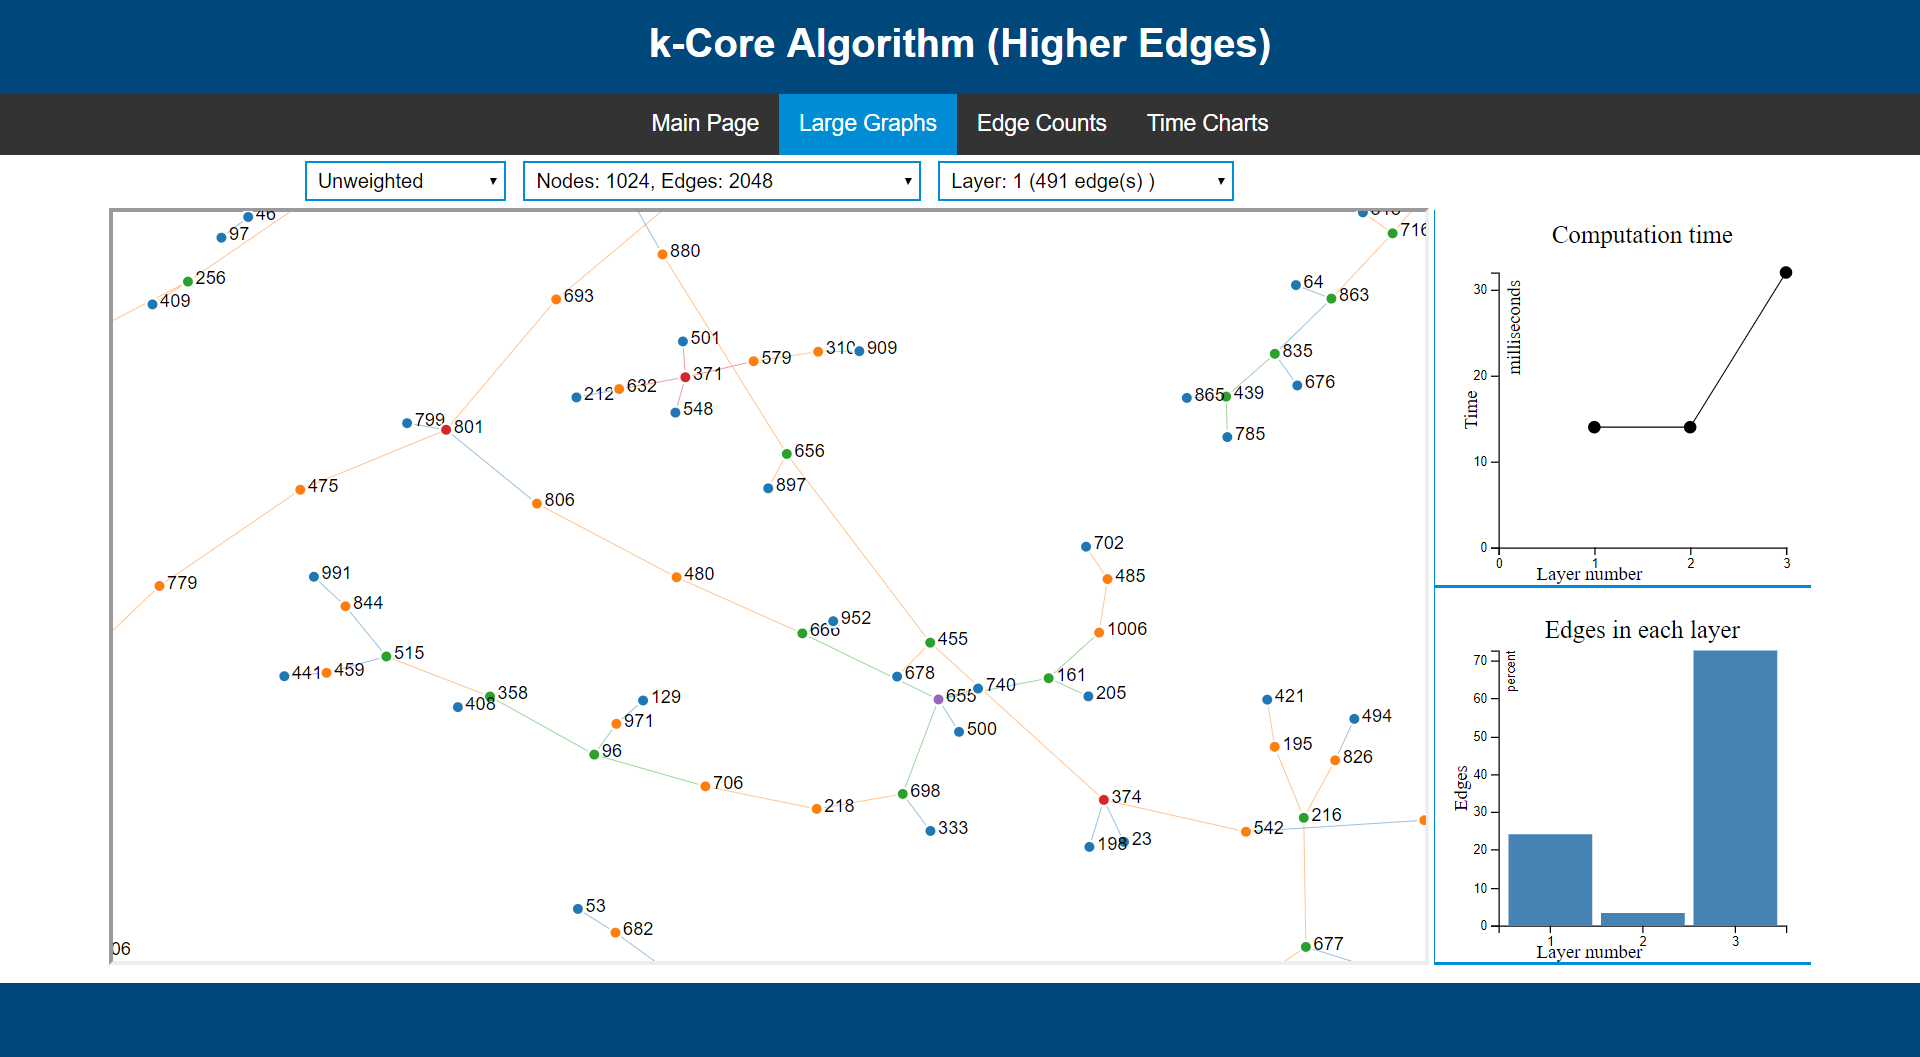
\includegraphics[width=8cm]{Large_Graphs.png}
    \end{center}
    \caption{ The Large Graphs Page }
    \end{figure}
    
    \item{\textit{Large Graphs Page:}}
    A graph with a large number of edges (in this case, $> 1024$) will have a large number of layers, and higher layers will also contain a large number of edges. To make it easier for the D3.js library to process these graphs and for the user to be able to view one layer at a time, a separate page is provided where these graphs and their layers can be viewed.
    \begin{itemize}
        \item The user can select between weighted and unweighted graphs.
        \item The user can then select the desired number of nodes and edges. The time-plot and edge concentration bar-graph will be displayed in the sidebar.
        \item When the graph is selected from the secondary drop down menu, a third selector will provide the choices of the graph's layers and also display the number of edges each of those graphs contain.
    \end{itemize}
        
    % \begin{figure}[!htbp]
    % \begin{center}
    % 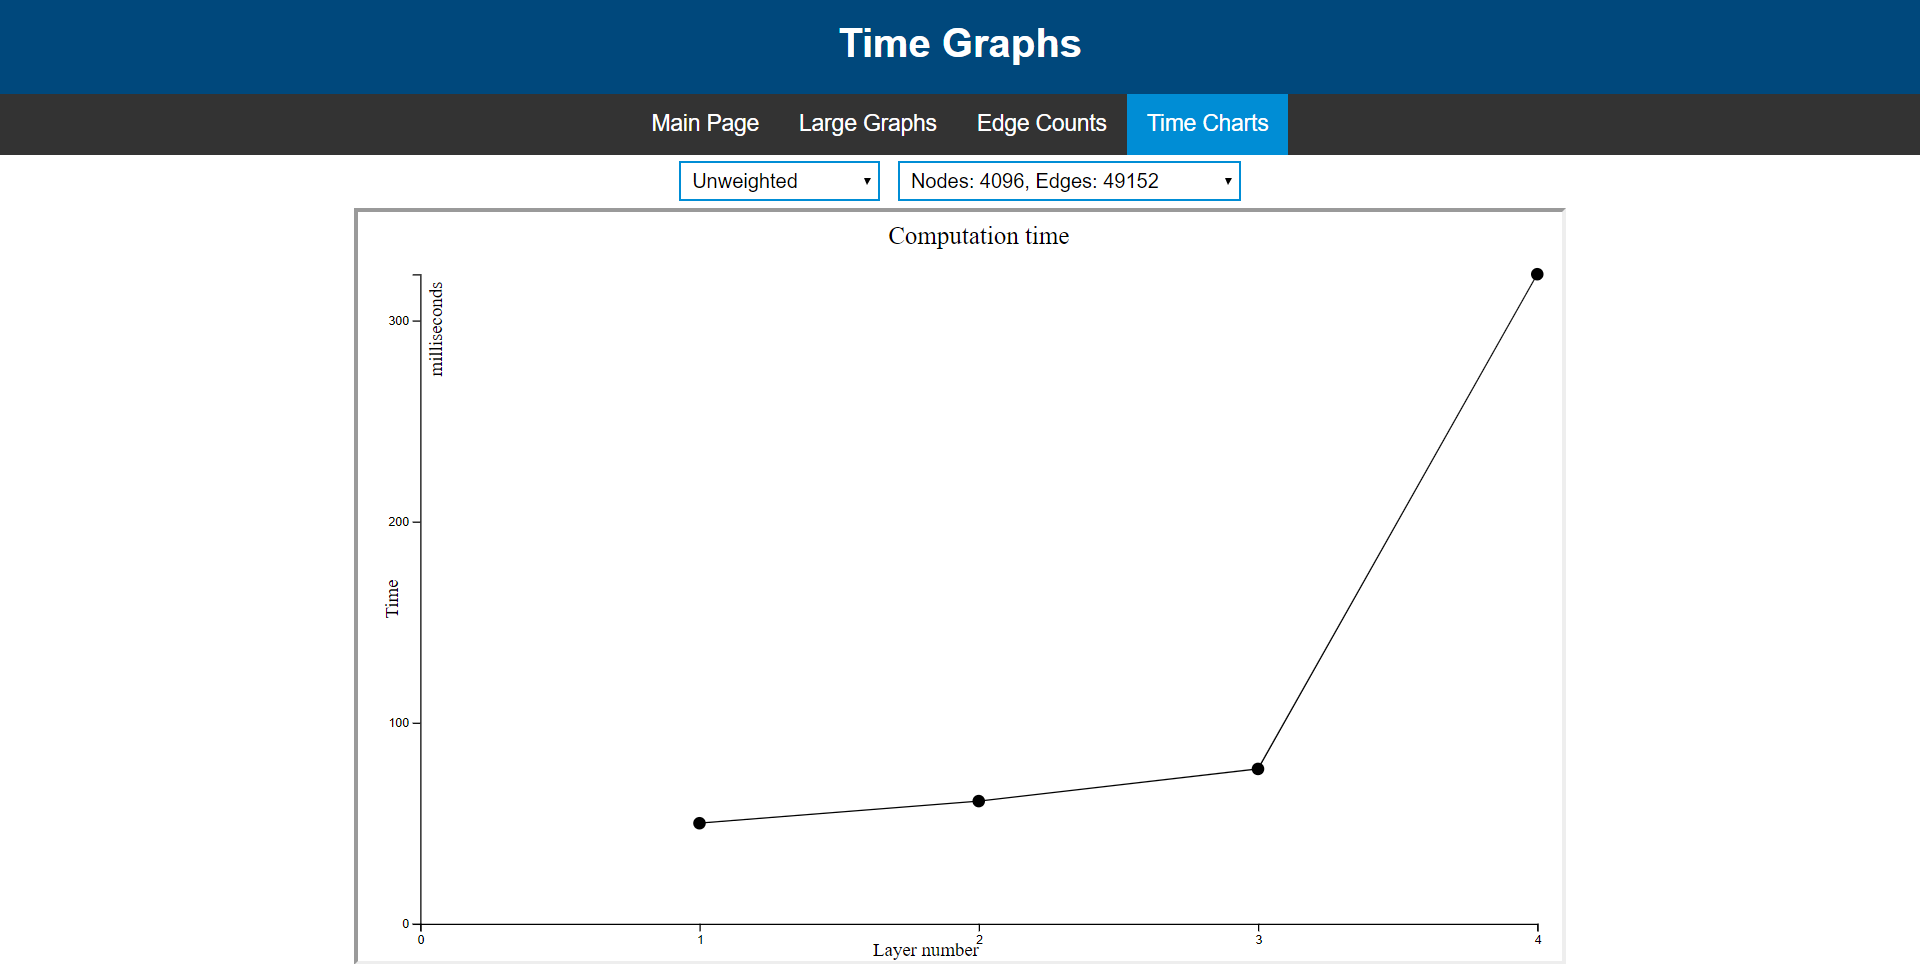
\includegraphics[width=8cm]{Time_Chart.png}
    % \end{center}
    % \caption{ The Time Plot }
    % \end{figure}
    
    % \begin{figure}[!htbp]
    % \begin{center}
    % 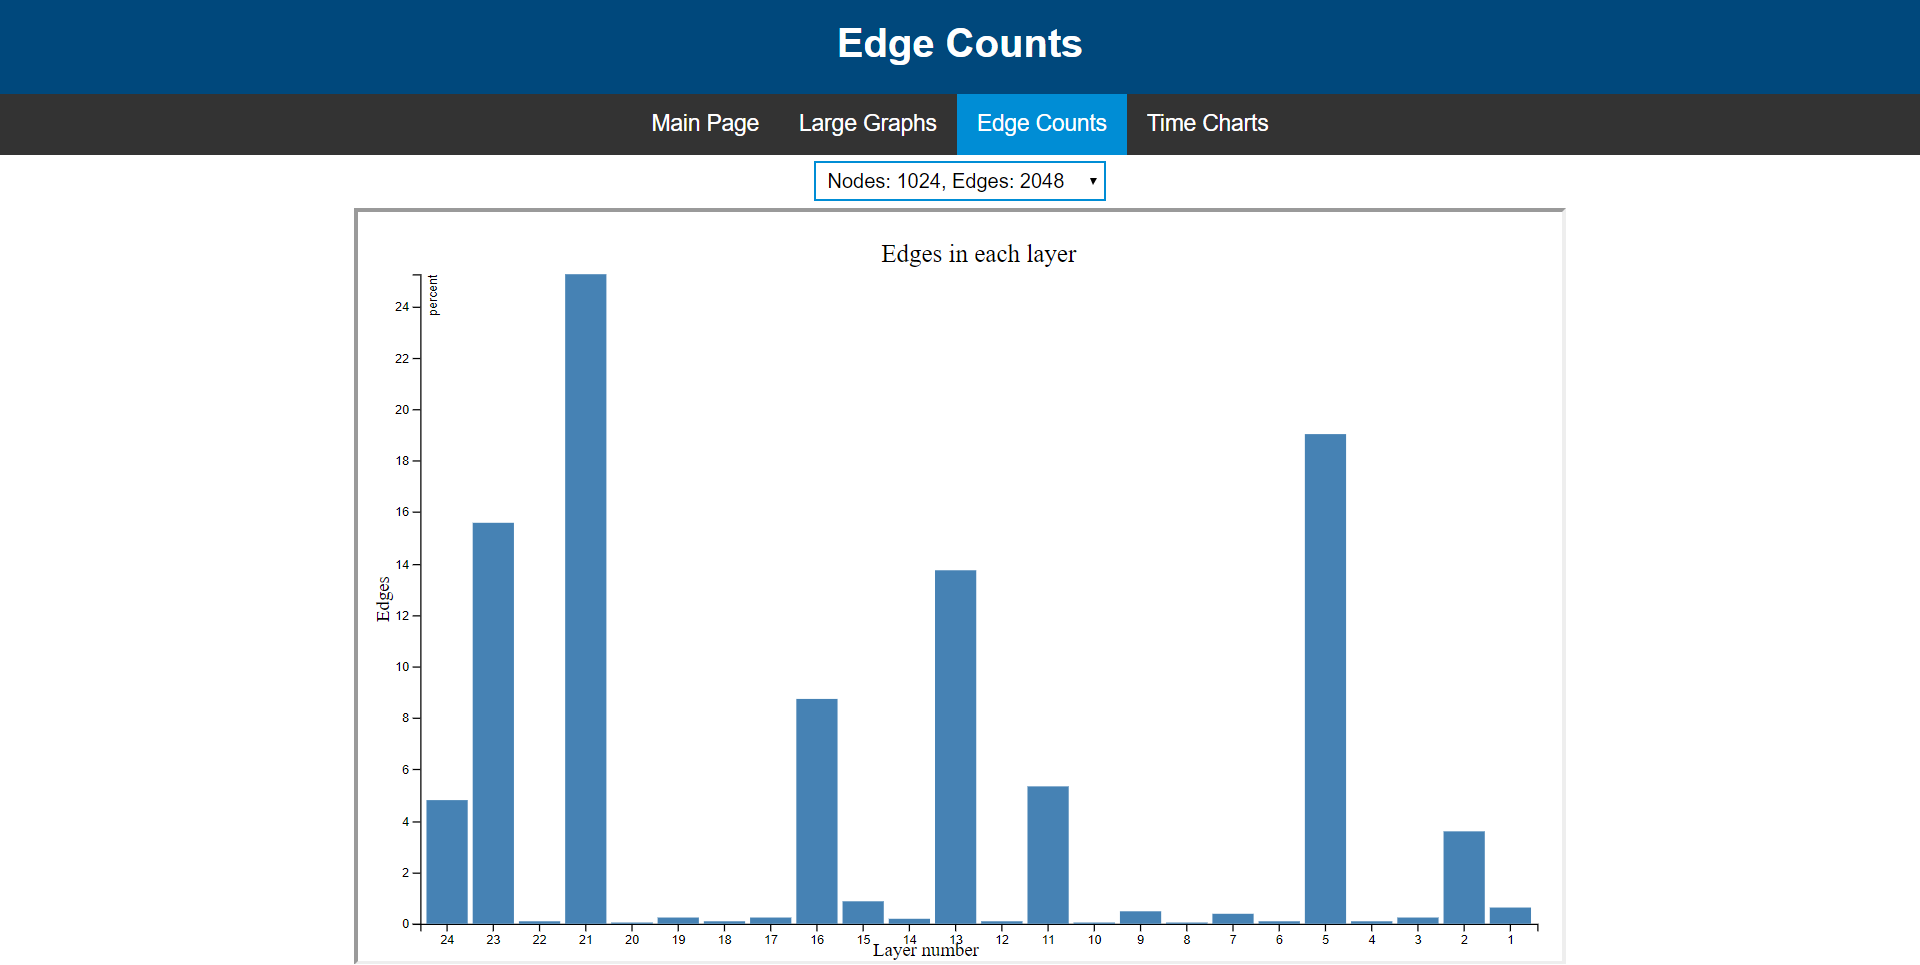
\includegraphics[width=8cm]{Edge_Concentration.png}
    % \end{center}
    % \caption{ The Edge Concentration Bar Graph }
    % \end{figure}
    
    \item For the convenience of the user, the plot for calculation time for each layer and the edge concentration bar graphs can be viewed in a larger window on separate pages.
    
\end{itemize}

